\begin{frame}[allowframebreaks]{Pipelines}
    \begin{itemize}
        \item A pipeline is a combination of data transformation and learning algorithms
        \item It has a \texttt{fit}, \texttt{predict}, and \texttt{score} method, just like any other learning algorithm
        \begin{itemize}
            \item Ensures that data transformations are applied correctly
        \end{itemize}
    \end{itemize}

    \begin{figure}
        \centering
        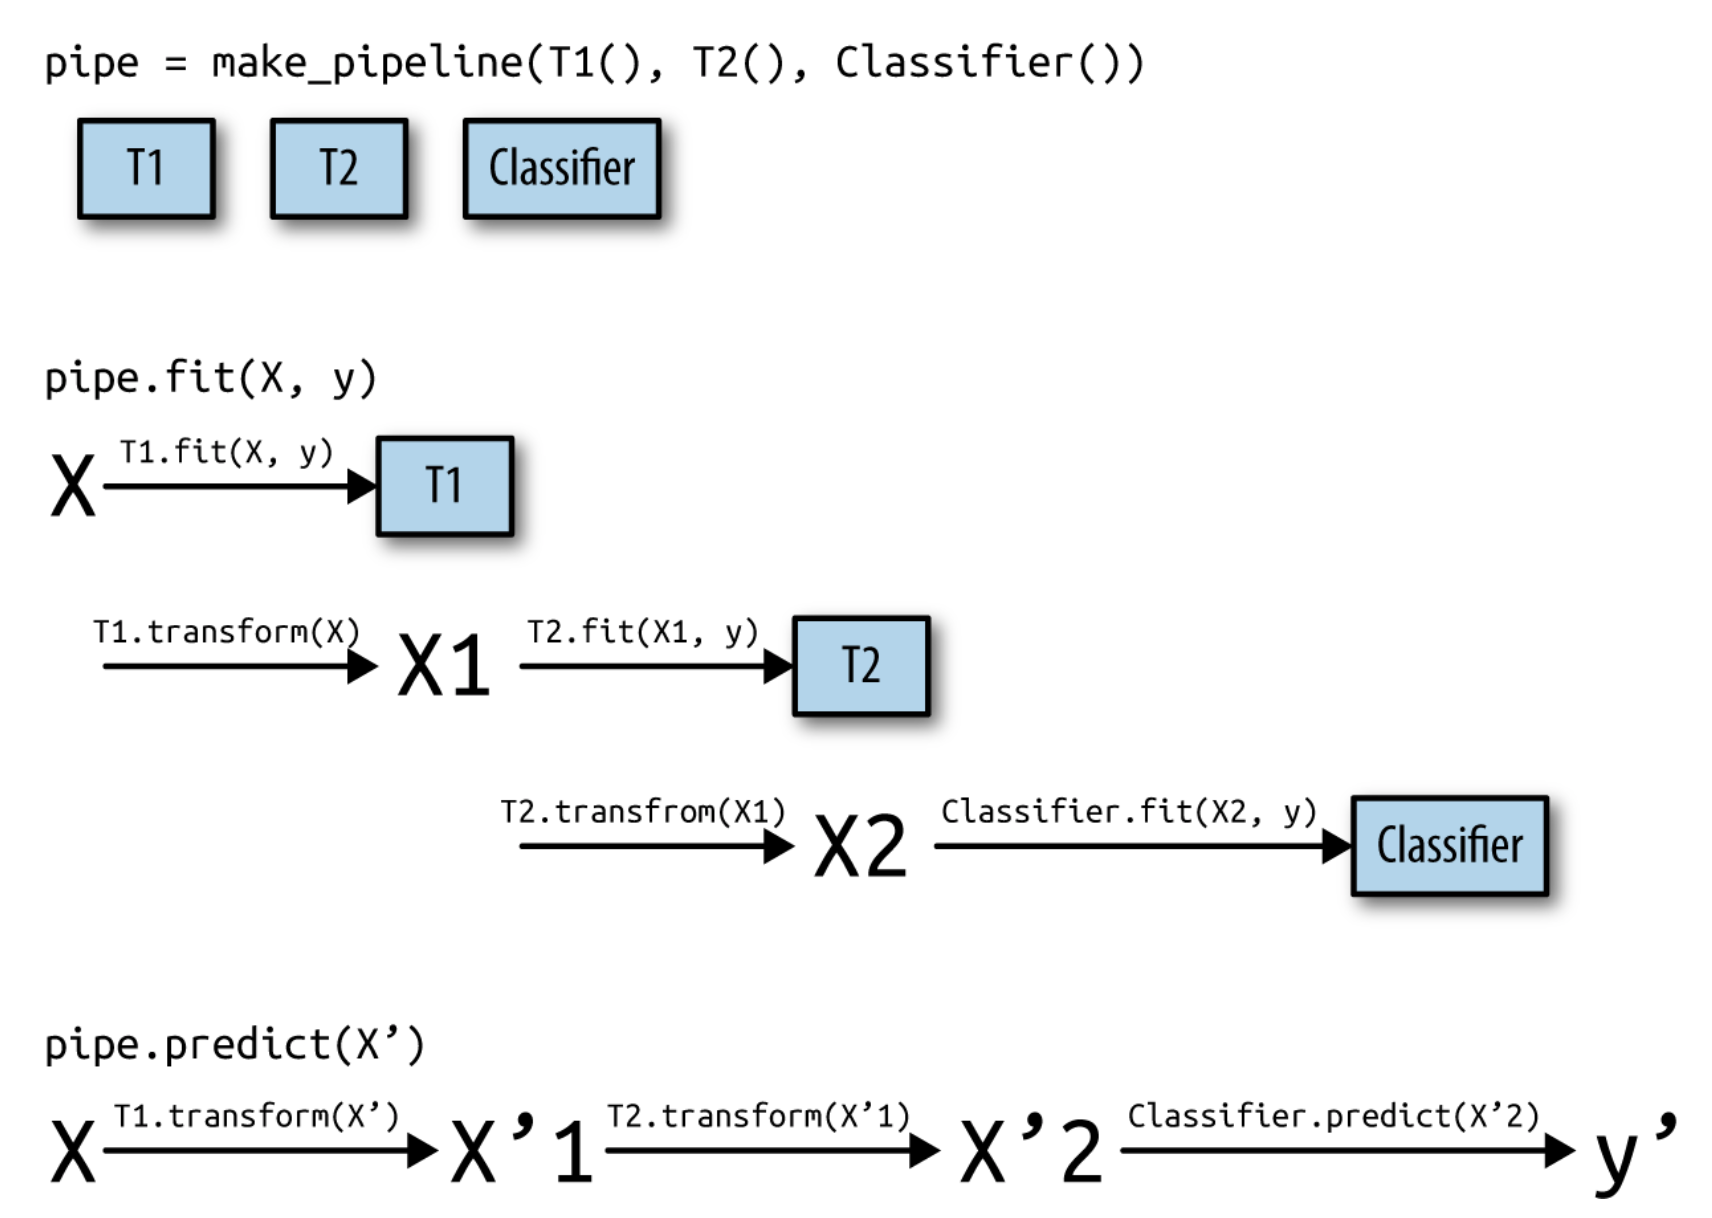
\includegraphics[width=0.95\textwidth,keepaspectratio]{images/pre-processing/pipeline.png}
    \end{figure}
\end{frame}

\begin{frame}[fragile]{In practice (scikit-learn)}
\begin{itemize}
    \item A \texttt{pipeline} combines multiple processing \textit{steps} in a single estimator
    \item All but the last step should be data transformer (have a \texttt{transform} method)
\end{itemize}

\vspace{1em}
\scriptsize
\begin{verbatim}
# Make pipeline, step names will be 'minmaxscaler' and 'linearsvc'
pipe = make_pipeline(MinMaxScaler(), LinearSVC())

# Build pipeline with named steps
pipe = Pipeline([("scaler", MinMaxScaler()), ("svm", LinearSVC())])

# Correct fit and score
score = pipe.fit(X_train, y_train).score(X_test, y_test)

# Retrieve trained model by name
svm = pipe.named_steps["svm"]

# Correct cross-validation
scores = cross_val_score(pipe, X, y)
\end{verbatim}
\normalsize
\end{frame}

\begin{frame}[fragile]{ColumnTransformer and FeatureUnion}
\begin{itemize}
    \item If you want to apply different preprocessors to different columns, use \texttt{ColumnTransformer}
    \item If you want to merge pipelines, you can use \texttt{FeatureUnion} to concatenate columns
\end{itemize}

\vspace{1em}
\scriptsize
\begin{verbatim}
# 2 sub-pipelines, one for numeric features, other for categorical ones
numeric_pipe = make_pipeline(SimpleImputer(), StandardScaler())
categorical_pipe = make_pipeline(SimpleImputer(), OneHotEncoder())

# Using categorical pipe for features A,B,C, numeric pipe otherwise
preprocessor = make_column_transformer((categorical_pipe,
                                        ["A", "B", "C"]),
                                        remainder=numeric_pipe)

# Combine with learning algorithm in another pipeline
pipe = make_pipeline(preprocessor, LinearSVC())
\end{verbatim}

\vspace{1em}
\begin{verbatim}
# Feature union of PCA features and selected features
union = FeatureUnion([("pca", PCA()), ("selected", SelectKBest())])
pipe = make_pipeline(union, LinearSVC())
\end{verbatim}
\normalsize
\end{frame}


\begin{frame}[fragile]{ColumnTransformer}
\begin{itemize}
    \item \texttt{ColumnTransformer} concatenates features in order
\end{itemize}

\vspace{1em}
\scriptsize
\begin{verbatim}
pipe = make_column_transformer((StandardScaler(), numeric_features),
                               (PCA(), numeric_features),
                               (OneHotEncoder(), categorical_features))
\end{verbatim}
\normalsize

\begin{figure}
    \centering
    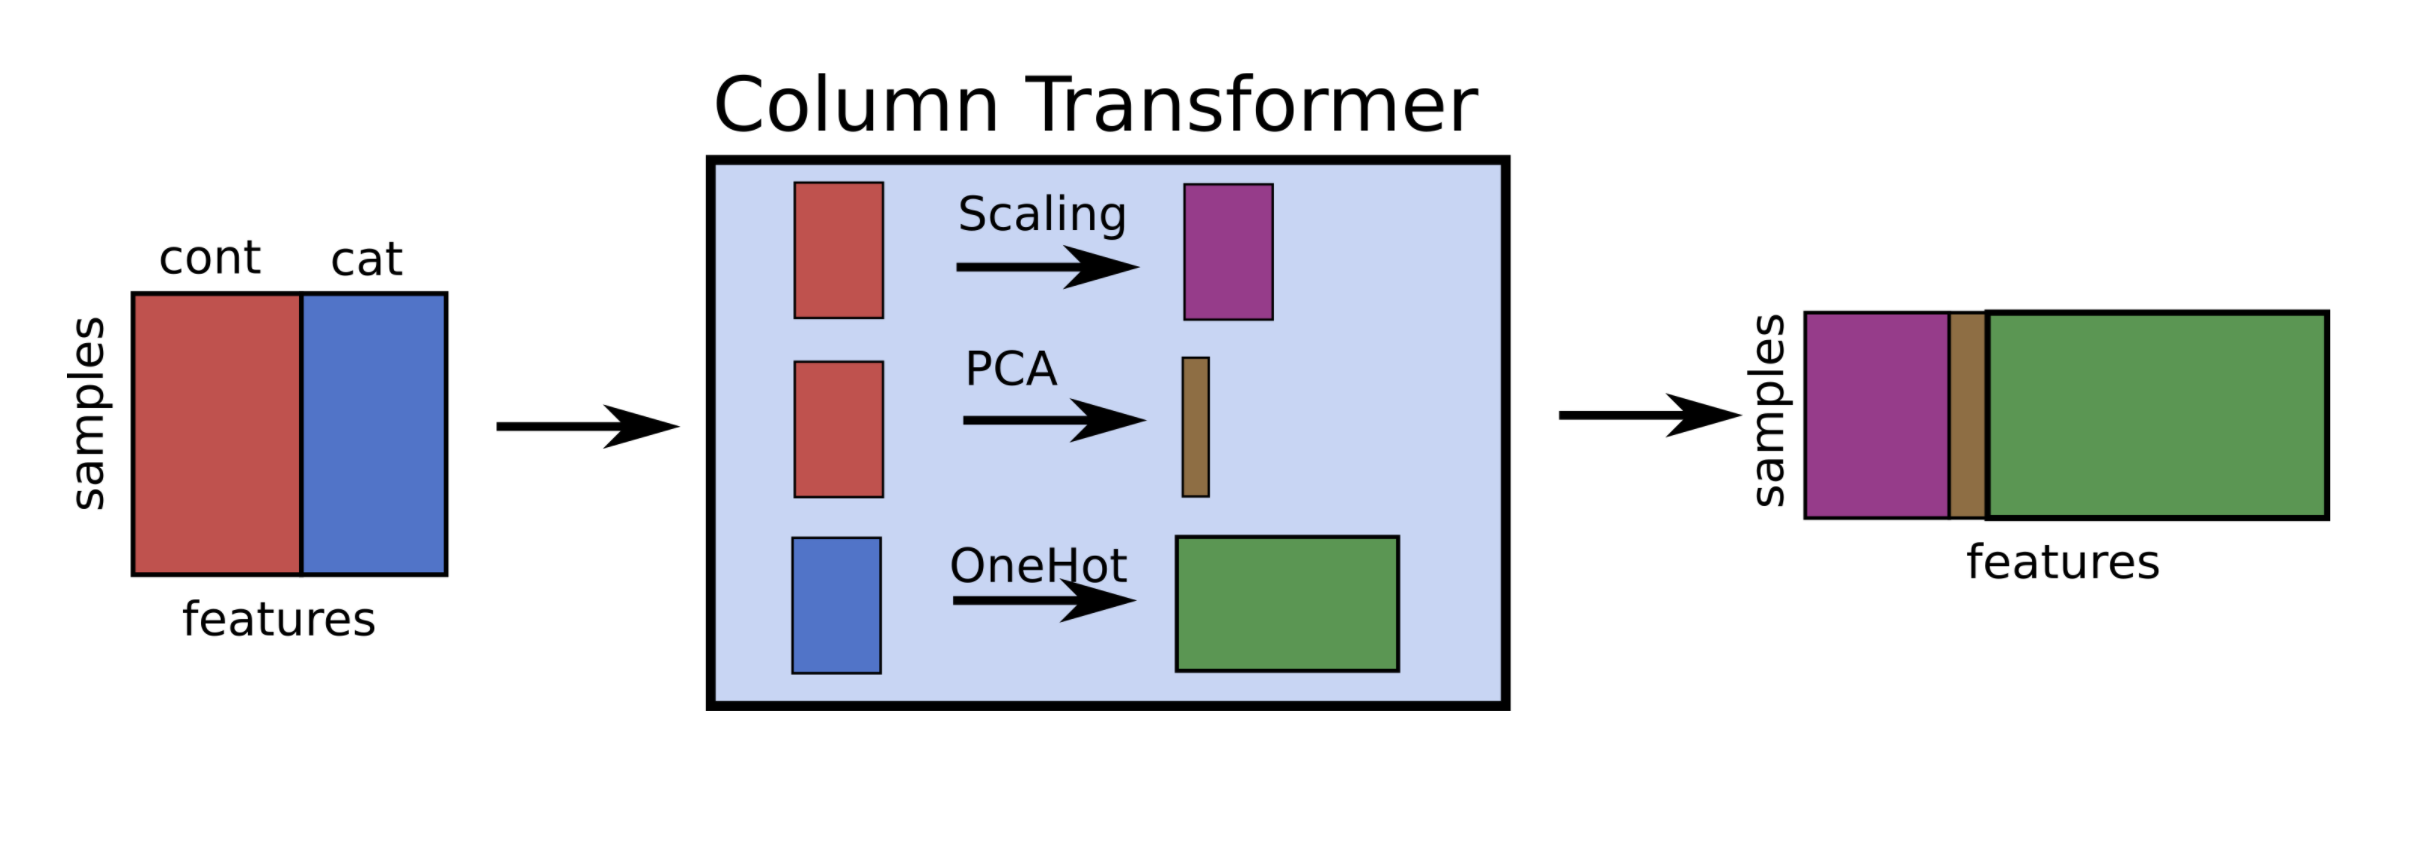
\includegraphics[width=0.9\textwidth,keepaspectratio]{images/pre-processing/columntransformer.png}
\end{figure}
\end{frame}


\begin{frame}[fragile]{Pipeline selection}
\begin{itemize}
    \item We can safely use pipelines in model selection (e.g. grid search)
    \item Use \texttt{\_\_} to refer to the hyperparameters of a step, e.g. \texttt{svm\_\_C}
\end{itemize}

\vspace{1em}
\scriptsize
\begin{verbatim}
# Correct grid search (can have hyperparameters of any step)
param_grid = {'svm__C': [0.001, 0.01],
              'svm__gamma': [0.001, 0.01, 0.1, 1, 10, 100]}
grid = GridSearchCV(pipe, param_grid=param_grid).fit(X, y)

# Best estimator is now the best pipeline
best_pipe = grid.best_estimator_
\end{verbatim}

\vspace{1em}
\begin{verbatim}
# Tune pipeline and evaluate on held-out test set
grid = GridSearchCV(pipe, param_grid=param_grid).fit(X_train, y_train)
grid.score(X_test, y_test)
\end{verbatim}
\normalsize
\end{frame}


\begin{frame}[fragile]{Example: Tune multiple steps at once}
\scriptsize
\begin{verbatim}
pipe = make_pipeline(StandardScaler(), PolynomialFeatures(), Ridge())
param_grid = {'polynomialfeatures__degree': [1, 2, 3],
              'ridge__alpha': [0.001, 0.01, 0.1, 1, 10, 100]}
grid = GridSearchCV(pipe, param_grid=param_grid).fit(X_train, y_train)
\end{verbatim}
\normalsize

\vspace{1em}
\begin{figure}
    \centering
    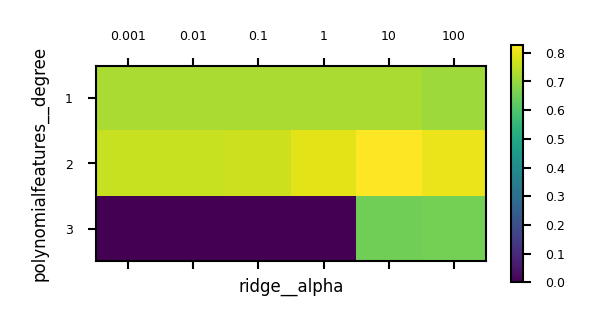
\includegraphics[width=0.8\textwidth,keepaspectratio]{images/pre-processing/pipeline_2.png}
\end{figure}
\end{frame}
